\section{Application isolation abstractions cause resource contention}
This section characterizes the performance of parallel applications under different levels of parallelism, paying particular attention to program behavior when parallelism is high. Based on this characterization, we argue that the exisiting isolation abstractions are inadequate for multi-tenant, highly parallel workloads.

While many classes of applications might benefit from cooperative resource sharing, this paper focuses its evaluation on highly parallel applications. We chose to focus on parallel applications because:
\begin{enumerate}
    \item Cloud computing workloads are commonly parallel. Due to trends in commodity hardware, parallellizing work will even more important in the future.
    \item Parallel workloads uniquely benefit from detailed knowledge of the underlying hardware. They would like to utilize all cores if possible, and often need to micro-optimize to maximize cache hits.
\end{enumerate}

When optimizing parallel programs, application developers must carefully balance the performance benefits of increased concurrency with the performance costs of interference between concurrent activities.

Therefore, deciding how much parallelism to introduce in a program is one of the most important decisions an application developer can make. While it is obvious why under-using parallelism sacrifices performance, the ``upper bound'' is less understood.

\begin{figure}[t!]
    \centering
    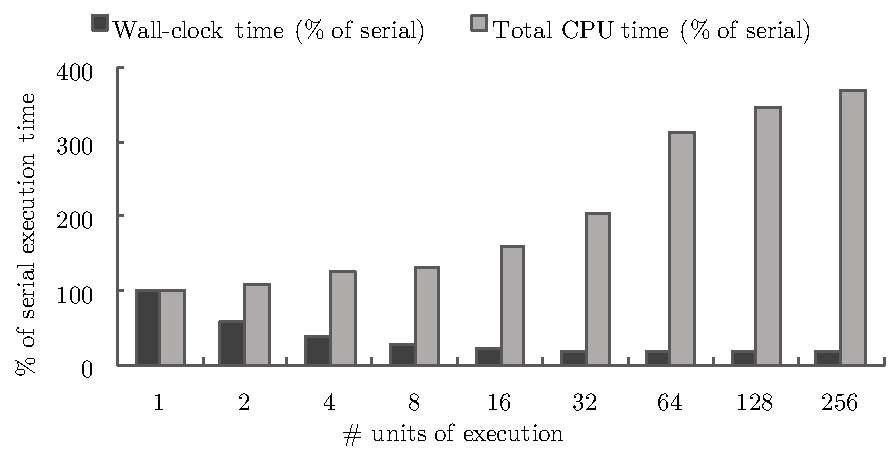
\includegraphics[width=8cm,height=4cm]{fig/speed-up.pdf}
    \caption{Wall-clock and total CPU execution times of the \texttt{bodytrack} application from the PARSEC benchmark suite~\cite{bienia2008parsec}. Increasing parallelism typically improves wall-clock execution time. However, total CPU time can increase, using more CPU resources to complete the same job. As an example, increasing from 16 to 32 threads increases total CPU time by approximately one-third, but we only see negligible improvement in wall-clock time.}
    \label{fig:speed-up}
\end{figure}

\subsection{Performance gains from parallelization are highly variable due to resource contention}
In a perfectly parallelizable workload, we would expect to see wall-clock execution speed up linearly with increasing parallelism. In real-world situations, however, wall-clock time typically speeds up sub-linearly with increasing parallelism (see Figure~\ref{fig:speed-up}).

\begin{figure}
\centering
  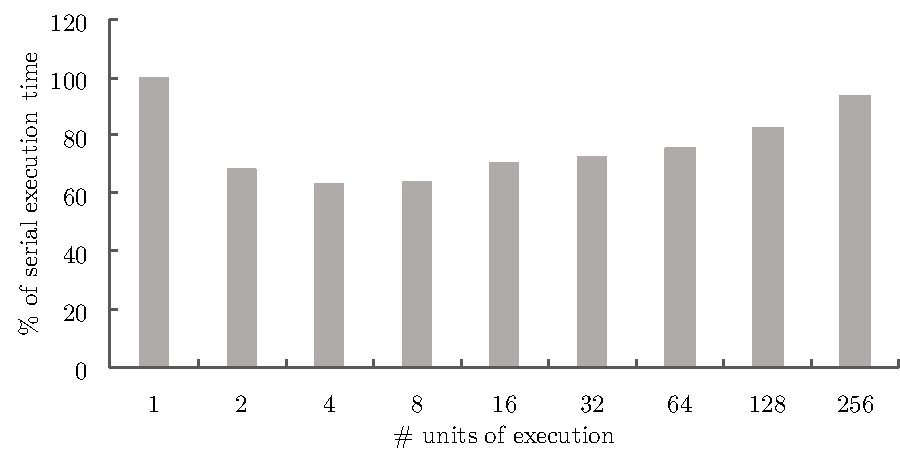
\includegraphics[width=8cm,height=4cm]{fig/contention.pdf}
  \caption{Wall-clock execution times for a job consisting of 16 instances of the PARSEC benchmark application \texttt{fluidanimate}. In each observation, we start the 16 instances simultaneously, all with the same number of threads (varied in along the x-axis). Parallel applications are designed to perform better with more units of execution, but performance can quickly degrade under contention.}
  \label{fig:contention-same}
\end{figure}

Clearly, increasing parallelism comes with costs. These costs are well documented, and include:
\begin{itemize}
  \item \textbf{Hardware resource contention.} CPU cores, main memory, bus throughput, etc. 
  \item \textbf{Context switch overhead.} Kernel time, cache invalidation, etc.
  \item \textbf{Synchronization overhead.} Common primitives (mutexes, semaphores, etc.) introduce overhead when contended for.
\end{itemize}

For most embarrassingly parallel problems, synchronization overhead is not high, as mutex contention is minimal. Context switch overhead can largely be reduced to a resource contention problem, as the cost of a context switch is dominated by cache invalidation~\cite{li2007quantifying}. Thus, we focus on the costs stemming from hardware resource contention.

\subsection{Isolation abstractions cannot solve resource contention}
We argue that the existing abstractions are inadequate for handling resource contention in multi-tenant, highly parallel workloads. The illusion of a single-user machine causes applications to systematically overuse finite hardware resources. As long as applications can expect to be ``greedy'' with regard to the hardware resource they are presented with, they will behave badly in multi-tenant environments (see Figure 2).

\subsubsection{Application doesn't know what resources it has}
In the existing scheme, user-level applications have the power to spawn threads and subprocesses, but little information about the state of hardware resources. Often, the degree of parallelism is statically determined by the application developer, with little regard for portability or the operating environment.

When the number of such applications on a given machine increases, the concurrent applications may not run efficiently. For example, on an Intel Xeon Phi processor with 64 cores, each supporting up to 4 hyperthreads, an application would create 256 threads for this hardware.  If its available hardware can only run a small number of threads because several applications are sharing the same machine, the overheads of 256 threads introduce inefficiency. 

% Figure  shows that the slowdowns of the PARSEC benchmark suite when using fewer number of CPU cores.  The worst case is XXX which slows down by a factor of 2 when running 256 threads on a single CPU core.

A common strategy to mitigate this problem to use a sophisticated dynamic parallelism library, such as Intel's TBB or Microsoft's TPL \cite{reinders2007intel}\cite{hellerstein2008optimizing}. However, this only performs optimization at the application level, running afoul of the scenario described above. Without understanding of the underlying resource environment, any application-local optimization cannot make globally optimal decisions.

\subsubsection{How applications are scheduled dramatically affects overall system performance}
The second reason is that the kernel does not have enough information to schedule multiple applications to maximize the efficiency or throughput of the hardware.  As an example, suppose an application has the following elapse times and speedups:
\begin{itemize}
\item
200 seconds on a single core.
\item 
12.5 seconds on 32 cores (16X speedup), with the best number of threads
for 32 cores
\item
10 seconds on 64 cores (20X speedup), with the best number of threads for 64 cores.
\end{itemize}

If the OS runs this application twice on the 64 core, one instance at a time, it will take 10 + 10 = 20 seconds.  However, if it runs two instances concurrently and each instance runs the best number of threads for 32 cores, it will take 12.5 seconds.  The throughput of the system improves by 37.5\%.

\subsection{Current trends in virtualization will exacerbate this issue}
Our arguments also apply to virtual machines and containers.  Virtual machine monitors provides virtualized hardware for an entire software stack including multiple operating systems.  Applications and their operating systems share the same abstractions as applications might on real hardware.

Containers provides isolated environments in a traditional operating systems rather than providing virtualized hardware. Within the context of a container environment, the abstractions between applications and their operating systems remain the same.

\begin{figure}[t!]
    \centering
    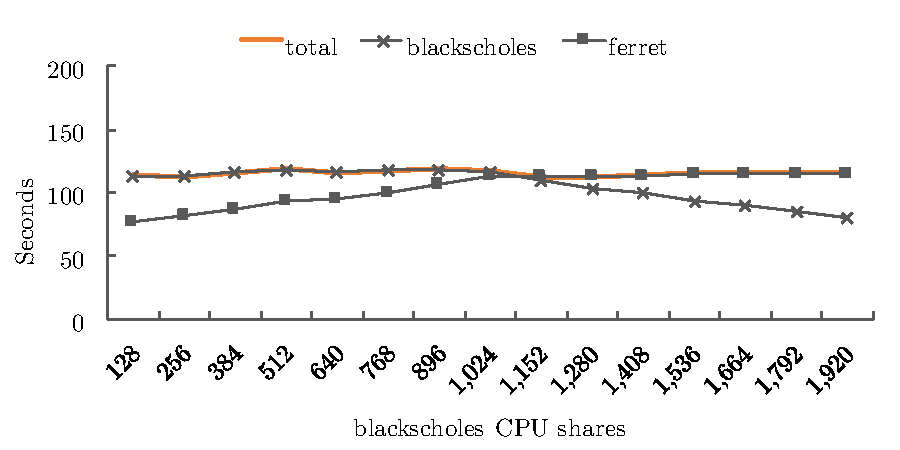
\includegraphics[width=8cm,height=4cm]{fig/without-application.pdf}
    \caption{Improving overall performance is difficult without true cooperation from applications.  In this simple example, we have a total of 2048 shares of CPU time that we divide among two applications, \texttt{blackscholes} and \texttt{ferret}, that start at the same time. We use Linux control groups to enforce that the two applications will have roughly the same ratio of time on CPU as the ratio of their weights. We can manipulate an application's resources with CPU shares, but we cannot alter application behavior via this mechanism and as a result, minimally impact the total execution time (orange, for those with color).}
    \label{fig:naive-cooperation}
\end{figure}